\documentclass[10pt, twocolumn]{article}

%-------------------------------------------------------------------------------
% PACKAGES
%-------------------------------------------------------------------------------
\usepackage[super]{natbib}
\usepackage{mathtools}
\usepackage{nameref}
\usepackage{fancyref}

% section numbering
\makeatletter
\def\@seccntformat#1{%
  \expandafter\ifx\csname c@#1\endcsname\c@section
  \fi}
\makeatother

% diagrams
\usepackage{tikz}
\usetikzlibrary{shapes,arrows,shadows}
\usepackage{amsmath,bm,times}
\newcommand{\mx}[1]{\mathbf{\bm{#1}}} % Matrix command
\newcommand{\vc}[1]{\mathbf{\bm{#1}}} % Vector command

%figures
\usepackage{caption}
\usepackage{subcaption}
\usepackage{epstopdf}
\usepackage{graphicx}
\graphicspath{{pictures/}}
\epstopdfsetup{outdir=pictures/}

%fancy stuff like color, paragraph formatting, code
\usepackage{hyperref}
\hypersetup{
     colorlinks   = true,
     citecolor    = gray
}
\usepackage{amsthm}

%one single command to rule them all references
\newcommand*{\fulleref}[1]{\hyperref[{#1}]{\autoref*{#1} \nameref*{#1}}} 
\usepackage{listings}
\usepackage{float}
\floatstyle{boxed}
\restylefloat{figure}


\title{
\includegraphics[scale=0.1]{logos} \vspace*{3\baselineskip}\\
        \large \textbf{\textsc{Master's Thesis}} \\
        \normalsize \textsc{University of Rennes 1} \\
        \normalsize \textsc{Bioinformatics and genomics Master's Degree} \\
        \normalsize \textsc{(2014 - 2015)} \vspace*{2\baselineskip} \\
		\large \textbf{\textsc{Test and benchmarking of a new scaffolding methodology}} \vspace*{0.5\baselineskip}\\
		\footnotesize \textsc{Institute for Research in IT and Random Systems, Genscale \\
		263 Avenue General Leclerc, 35000 Rennes, France}
        }
\author{\normalsize
	\begin{minipage}{0.4\textwidth}
	\begin{flushleft} 
	\emph{Author:}\\
	\textsc{Alexandrina Bodrug}
	\end{flushleft}
	\end{minipage}
	~
	\begin{minipage}{0.4\textwidth}
	\begin{flushright}
	\emph{Supervisors:} \\
	\textit{Pr.} \textsc{Univ. Rennes 1 Rumen Andonov} \\
	\textit{Dr.} \textsc{Cnrs Dominique Lavenier}
	\end{flushright}
	\end{minipage}\\[2cm]}
\date{\small \textsc{22 June, 2015}}
\begin{document}
\maketitle
\thispagestyle{empty}
\clearpage
%-------------------------------------------------------------------------------
% THX
%-------------------------------------------------------------------------------
\onecolumn
Thanks \\
\thispagestyle{empty}
\clearpage
%-------------------------------------------------------------------------------
% ABBRV	 & GITHUB
%-------------------------------------------------------------------------------
\onecolumn
Abbreviations \& github link
\thispagestyle{empty}
\clearpage
%-------------------------------------------------------------------------------
% ToC
%-------------------------------------------------------------------------------
\hypersetup{linkcolor=gray}
\tableofcontents
\thispagestyle{empty}
\newpage
%-------------------------------------------------------------------------------
% BODEH!
%-------------------------------------------------------------------------------
\twocolumn
\section{Introduction}
\setcounter{page}{1}
\subsection{Backgroud}
\textit{De novo} assembly is the process which pieces together overlapping small fragmented DNA sequences produced by Next Generation Sequencing methods into larger sequences. The aim is to obtain complete genomes (or chromosomes) containing gaps of known lengths because the less fragmented the genome is, the easier the downstream analysis are \cite{hunt_comprehensive_2014}. However an incomplete assembly is still sufficient for most of the analysis performed on DNA which explains why databases mainly contain partially assembled genomes. Nonetheless the uninterrupted genome sequence is a precious information and there has been an important effort made to improve the performance of assembly algorithms and the quality of NGS data. The the detailed process of assembly is described in ~\fulleref{sec:assterm}; the two main steps are building contigs from reads (sometimes referred to as assembly) and scaffolding, the ordering and relative orientation of contigs or unitigs. The 2011 and 2013 Assemblathon projects \cite{earl_assemblathon_2011} \cite{bradnam_assemblathon_2013} aimed at  benchmarking existing assembly tools with high coverage diploid genomes. The studies focused mainly on the contig building step, concluding that although many tools found quality assemblies, the tool and quality criteria should be adjusted to the type of genome and the goal of the assembly project. For example a good N50, an extensively used metric which is the contig length such that using equal or longer contigs produces half the bases of the genome, is not essential in a gene detecting assembly project. \\
The first stand-alone scaffolder named Bambus \cite{pop_hierarchical_2004}, originally part of the MetAMOS \cite{treangen_metamos:_2013} assembly and analysis pipeline, was published in 2004. Previously the scaffolding step was missing or presented as an option within conting builders, for instance the Velvet\cite{zerbino_velvet:_2008} assembler \textit{'scaffolding yes or no'} option. In the 2014 comprehensive evaluation of scaffolding tools \cite{hunt_comprehensive_2014-1}, Hunt \textit{et al} found that no tool identified more than 90\% of joins between real-data Velvet assembled contigs, meaning genomes were still fragmented into many scaffolds as joins were missing for a complete and accurate ordering and orientation. The study also used simulated data highlighting the fact that perfect data doesn't always yield perfect results. Despite its simply formulated goal - order and orient contigs - scaffolding is a challenging computational problem. It was first described and modeled in 2002 by Hudson \textit{et al.}\cite{huson_greedy_2002} which proposed a greedy path-merging strategy, described in \fulleref{sec:hiscaf} along with other proposed algorithms.
 
\subsection{Assembly terminology}\label{sec:assterm}
In this report \textit{assembly} will refer to the whole multi-step process which starts from once filtered out-of-the-sequencer data and results, in the best case scenarios, in  highly uninterrupted sequence of a genome or chromosome. As previously mentioned, the two main steps are contig/unitig building and contig/unitg scaffolding. The difference between contig and unitig is fundamental to understanding the Genscale scaffolding challenges. Another key point is the construction of joins between contigs/unitigs - also referred to as links, edges, bonds \ldots 
\subsubsection{Reads, pairing and overlaps} \label{sec:rpao}

A read is a short ($<500pb$) copy of a DNA fragment of known length and nucleic acid order. It is produced differently depending of the sequencing technology. Paired reads are copies of the two extremities of a DNA molecule. The DNA sequence between two reads of a pair is called an insert. The size of the insert is variable. Reads with small insert sizes ($<500bp$) are called paired-end reads. Mate-paired reads are reads whose insert size is very big (up to tens of kilobases). The pairing information and the size of the insert are provided by the sequencer. A collection of reads with their associated insert size is called a a genomic library.
\begin{figure}[h!]
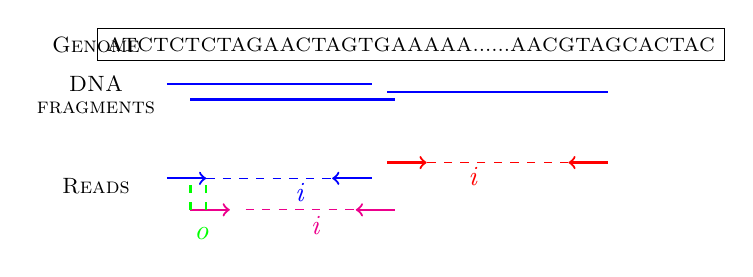
\begin{tikzpicture}
\node[draw=none] at (-4,0) {\footnotesize \textsc{Genome}};
\node[draw] at (0,0) {\scriptsize ATCTCTCTAGAACTAGTGAAAAA......AACGTAGCACTAC};
\node[draw=none] at (-4,-0.5) {\footnotesize \textsc{DNA}};
\node[draw=none] at (-4,-0.8) {\footnotesize \textsc{fragments}};
\draw[thick, blue] (-3.1, -0.5) -- (-0.5, -0.5);
\draw[thick, blue] (-0.3, -0.6) -- (2.5, -0.6);
\draw[thick, blue] (-2.8, -0.7) -- (-0.2, -0.7);
\node[draw=none] at (-4,-1.8) {\footnotesize \textsc{Reads}};

\draw[red, thick, <-] (2,-1.5) -- (2.5,-1.5);
\draw[red, dashed] (2,-1.5) -- (0.2,-1.5);
\node[draw=none, color=red] at (0.8,-1.68) {\textit{i}};
\draw[red, thick, ->] (-0.3,-1.5) -- (0.2,-1.5);

\draw[blue, thick, <-] (-1,-1.7) -- (-0.5,-1.7);
\draw[blue, dashed] (-2.6,-1.7) -- (-1,-1.7);
\node[draw=none, color=blue] at (-1.4,-1.88) {\textit{i}};
\draw[blue, thick, ->] (-3.1,-1.7) -- (-2.6,-1.7);

\draw[magenta, thick, <-] (-0.7,-2.1) -- (-0.2,-2.1);
\draw[magenta, dashed] (-2.1,-2.1) -- (-0.7,-2.1);
\node[draw=none, color=magenta] at (-1.2,-2.3) {\textit{i}};
\draw[magenta, thick, ->] (-2.8,-2.1) -- (-2.3,-2.1);

\node[draw=none, color=green] at (-2.65, -2.4) {\textit{o}};
\draw[green, dashed, thick] (-2.8, -2.1) -- (-2.8, -1.7); 
\draw[green, dashed, thick] (-2.6, -2.1) -- (-2.6, -1.7);
\end{tikzpicture}
\caption{Alignment of paired reads on fragmented DNA}
\label{fig:reads}
{\footnotesize  Each end of a DNA molecule is cloned to produce paired reads. Here is represented a mate-paired pair (red) with a big insert size \textit{(i)} and two paired-end pairs (blue and magenta) which slightly overlap \textit{(o)}. }
\end{figure}\\
Figure \ref{fig:reads} represents three pairs of reads. Within the pairs, reads are facing each other: this configuration is called \textit{Forward-Reverse} read orientation. To be sequenced the genome represented in figure \ref{fig:reads} is first amplified by Polymerase Chain Reaction and then fragmented into numerous DNA molecules by sonication or nebulization. Each end of the molecule is then cloned. Overlapping of reads occurs when two reads sequence a portion of the same genomic region, but not only. The overlapping concept implies a common origin but unfortunately overlapping can occur if two reads sequence two different repeated genomic regions. Figure \ref{fig:overlapping} shows how repeated regions create false positive overlaps. Such reads can be detected and filtered out by ignoring high-frequency overlaps (higher than the coverage at which the genome was sequenced). However this can result in false negatives and makes the task of assembling repeated regions very hard.
\begin{figure}[h!]
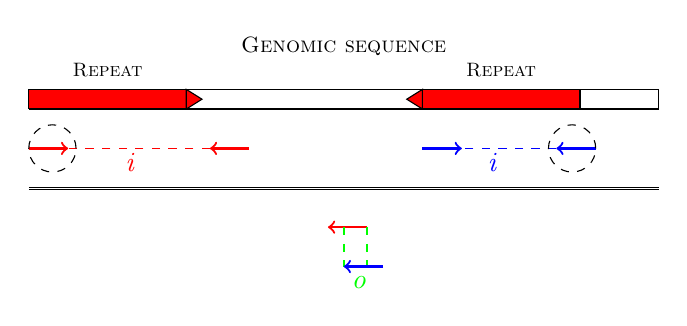
\begin{tikzpicture}
\node[draw=none] at (4,0.8) {\footnotesize \textsc{Genomic sequence}};
\node[draw=none] at (1,0.5) {\scriptsize \textsc{Repeat}};
\node[draw=none] at (6,0.5) {\scriptsize \textsc{Repeat}};
\draw[fill=red] (0,0) -- (2,0) -- (2,0.25) -- (0,0.25) -- (0,0);
\draw[fill=red] (2,0) -- (2,0.25) -- (2.2,0.125) -- (2,0);
\draw (2,0) -- (5,0) -- (5,0.25) -- (2,0.25) -- (2,0);
\draw[fill=red] (5,0) -- (5,0.25) -- (4.8,0.125) -- (5,0);
\draw[fill=red] (5,0) -- (7,0) -- (7,0.25) -- (5,0.25) -- (5,0);
\draw (7,0) -- (8,0) -- (8,0.25) -- (7,0.25) -- (7,0);

\draw[red, thick, <-] (2.3,-0.5) -- (2.8,-0.5);
\draw[red, dashed] (2.3,-0.5) -- (0.2,-0.5);
\node[draw=none, color=red] at (1.3,-0.68) {\textit{i}};
\draw[red, thick, ->] (0,-0.5) -- (0.5,-0.5);

\draw[blue, thick, <-] (6.7,-0.5) -- (7.2,-0.5);
\draw[blue, dashed] (6.7,-0.5) -- (5.2,-0.5);
\node[draw=none, color=blue] at (5.9,-0.68) {\textit{i}};
\draw[blue, thick, ->] (5,-0.5) -- (5.5,-0.5);

\draw[dashed] (0.3,-0.5) circle (0.3) ; 
\draw[dashed] (6.9,-0.5) circle (0.3) ; 

\draw (0,-1)-- (8,-1) ;
\draw (0,-1.02)-- (8,-1.02) ;

\draw[red, thick, ->] (4.3,-1.5) -- (3.8,-1.5);
\draw[green, thick, dashed] (4, -1.5) -- (4, -2);
\draw[green, thick, dashed] (4.3, -1.5) -- (4.3, -2);
\draw[blue, thick, ->] (4.5,-2) -- (4,-2);
\node[draw=none, color=green] at (4.2, -2.2) {\textit{o}};

\end{tikzpicture}
\caption{Overlapping induced by repeated sequences}
\label{fig:overlapping}
{\footnotesize  The two circled reads will have a significantly long and accurate overlap to imply a common genomic origin when in fact they come from distant regions.}
\end{figure}

\subsubsection{Unitigs and Contigs}
Unitigs, also sometimes called chunks, are an uniquely assemblable subset of overlapping fragments. At the end of an unitig data shows multiple dubious overlaps as seen in \fulleref{sec:rpao} creating joins with multiple other unitigs. Contigs are larger than unitigs, extended through repeat boundaries but are still ungapped sequences. Contigs are interesting to construct because there is a higher chance to detect genes, despite the risk of misassemblies and chimeric sequences. 
Taking the example shown in figure \ref{fig:overlapping}, a contig could cover all the green repeated area and afterwards be extended though ambiguous overlaps on both sides. Unitigs however will stop at the end of the green areas. In a sense, unitigs are either an unambiguous contig or a compression of several copies of a repeat. See example in figyre \ref{fig:unitgscontigs}.
\begin{figure}[h!]
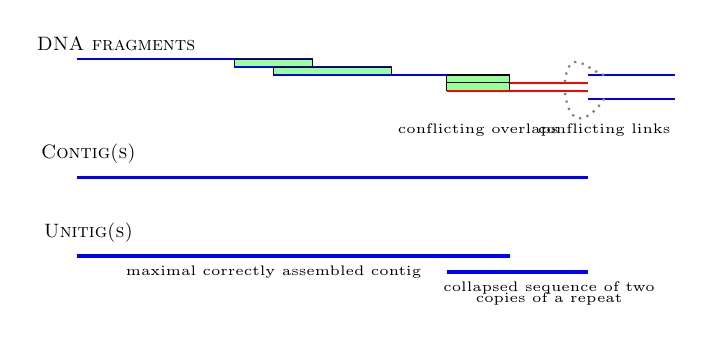
\begin{tikzpicture}
\node[draw=none] at (1,0.2) {\scriptsize \textsc{DNA fragments}};
\draw[thick, blue] (0.5,0) -- (3.5,0);
\draw[fill=green!40] (2.5,0) -- (3.5,0) -- (3.5,-0.1) -- (2.5,-0.1) -- (2.5,0);
\draw[thick, blue] (2.5,-0.1) -- (4.5,-0.1);
\draw[fill=green!40] (3,-0.1) -- (4.5,-0.1) -- (4.5,-0.2) -- (3,-0.2) -- (3,-0.1);
\draw[thick, blue] (3.0,-0.2) -- (6.0,-0.2);
\draw[fill=green!40] (5.2,-0.2) -- (6.0,-0.2) -- (6.0,-0.3) -- (5.2,-0.3) -- (5.2,-0.2);
\draw[thick, red] (5.2,-0.3) -- (7,-0.3);
\draw[fill=green!40] (5.2,-0.3) -- (6.0,-0.3) -- (6.0,-0.4) -- (5.2,-0.4) -- (5.2,-0.3);
\draw[thick, red] (5.2,-0.4) -- (7,-0.4);
%\draw[fill=green!40] (7.0,-0.4) -- (7.5,-0.4) -- (7.5,-0.5) -- (7.0,-0.5) -- (7.0,-0.4);
\draw[thick, blue] (7.0,-0.5) -- (8.1,-0.5);
%\draw[fill=green!40] (7.0,-0.2) -- (7.5,-0.2) -- (7.5,-0.3) -- (7.0,-0.3) -- (7.0,-0.2);
%\draw[fill=green!40] (7.0,-0.3) -- (7.5,-0.3) -- (7.5,-0.4) -- (7.0,-0.4) -- (7.0,-0.3);
\draw[thick, blue] (7.0,-0.2) -- (8.1,-0.2);

\draw[color=gray, dotted, thick] (7.2,-0.2) .. controls  (7,-0.15) and (6.75,0.2) .. (6.7,-0.3);
\draw[color=gray, dotted, thick] (7.2,-0.5) .. controls  (7,-0.8) and (6.75,-0.9) .. (6.7,-0.4);

\node[draw=none] at (5.6,-0.9) {\tiny conflicting overlaps};
\node[draw=none] at (7.2,-0.9) {\tiny conflicting links};
\node[draw=none] at (0.65,-1.2) {\scriptsize \textsc{Contig(s)}};
\draw[very thick, blue] (0.5, -1.5) -- (7, -1.5);
\node[draw=none] at (0.65,-2.2) {\scriptsize \textsc{Unitig(s)}};
\draw[very thick, blue] (0.5, -2.5) -- (6.0, -2.5);
\node[draw=none] at (3,-2.7) {\tiny maximal correctly assembled contig};
\draw[very thick, blue] (5.2, -2.7) -- (7, -2.7);
\node[draw=none] at (6.5,-2.9) {\tiny collapsed sequence of two };
\node[draw=none] at (6.5,-3.05) {\tiny copies of a repeat};
\end{tikzpicture}
\caption{The difference between unitigs and contigs}
\label{fig:unitgscontigs}
{\footnotesize Unitigs end at multiple overlaps indicating a possible repeat. Contigs can be extended through conflicting overlaps. Here, the red DNA fragments are two copies of a repeat. When no more overlaps exist, contigs can be linked (gray dotted line) thanks to information provided by read pairs. This is the scaffolding task. Here alternative paths are possible due to the repeated region.}
\end{figure}
 
\subsubsection{Scaffolding and obtaining a consensus sequence}
A scaffold is a linear ordering of contigs (or unitigs). The ordering and relative orientation of contigs is possible thanks to paired reads information. The first step of scaffolding is mapping reads on the previously constructed reads: the two most used mappers are bwa \cite{li_fast_2009} and bowtie\cite{langmead_fast_2012,langmead_ultrafast_2009}. A pair of reads mapping on two different contigs provide a join, which holds the information of distance between the two contigs, and relative orientation (see figure \ref{fig:mappreads} ). The concept of insert size is essential to understand the challenges of scaffolding. 
\begin{figure}[h!]
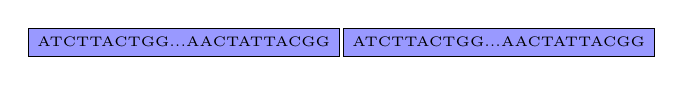
\begin{tikzpicture}
%\node[draw=none] at (1,0.2) {\scriptsize \textsc{Contigs}};
\node[draw, fill=blue!40] at (0,-0.5) {\tiny ATCTTACTGG...AACTATTACGG};
\node[draw, fill=blue!40] at (4,-0.5) {\tiny ATCTTACTGG...AACTATTACGG};

\end{tikzpicture}
\caption{Creating joins between contigs thanks to read-pair information}
\label{fig:mappreads}
{\footnotesize Note}
\end{figure}



\subsection{A history of scaffolding strategies}\label{sec:hiscaf}
The contig scaffolding problem was first introduced in 2002 by Hudson and al. \cite{huson_greedy_2002} following the challenges which arose during the clone-bt-clone Whole Genome Project and whole genome shotgun assembly project. 
Most tools model the problem as a graph where vertices represent contigs and links represent bundles of pairs of reads linking two contigs. Erroneous data (fake links due to poorly assembled contigs, low quality libraries), missing data (low quality libraries, unfit insert size, low genome coverage) and inherent genome characteristics (repeated regions,  heterozygosity) stand in the way of a perfect and easy scaffolding process.
\subsection{Context and goal of the internship project}


\iffalse
notes
\fi
%-------------------------------------------------------------------------------
% BODEH!
%-------------------------------------------------------------------------------
\section{Material and methods}
\subsection{Input data for genscale scaffolders}
The input data for the genscale scaffolders contains a list of unitigs and a list of links between unitigs. 
\subsubsection{Format}
\subsubsection{Methods}
\subsection{Features of the assembled genomes}
\subsubsection{Chloroplasts}
Chloroplasts are small organelles in plant photosynthetic tissues which possess their own DNA. The chloroplast genomes are small ($\approx 150kpb$), circular and have a large inverted repeated sequence of around $25kpb$. 
\begin{figure}[h!]
\centering
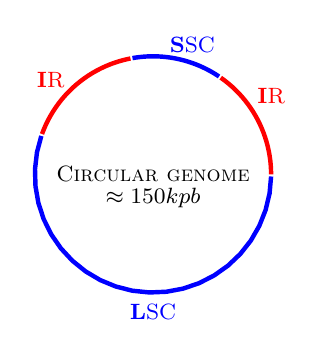
\begin{tikzpicture}
   \draw [red,ultra thick,domain=0:55] plot ({1.5*cos(\x)}, {1.5*sin(\x)});
   \draw [blue,ultra thick,domain=56:100] plot ({1.5*cos(\x)}, {1.5*sin(\x)});
   \draw [red, ultra thick, domain=101:160] plot ({1.5*cos(\x)}, {1.5*sin(\x)});
   \draw [blue, ultra thick, domain=161:359] plot ({1.5*cos(\x)}, {1.5*sin(\x)});
   \node[draw=none, fill=none] at (0,0) {\footnotesize \textsc{Circular genome }};
   \node[draw=none, fill=none] at (0,-0.3) {\footnotesize $\approx 150kpb$};
   \node[draw=none, fill=none] at (1.5,1) {\footnotesize \color{red} \textbf IR};
   \node[draw=none, fill=none] at (-1.3,1.2) {\footnotesize \color{red} \textbf IR};
   \node[draw=none, fill=none] at (0,-1.75) {\footnotesize \color{blue} \textbf LSC};
   \node[draw=none, fill=none] at (0.5,1.65) {\footnotesize \color{blue} \textbf SSC};
\end{tikzpicture}
\caption{Chloroplast genome structure}
{\footnotesize Inverted Repeat (IR $ \approx 23kpb$) ; Long Single Copy (LSC); Small Simple Copy (SSC $\approx 85kpb$)}
\end{figure} \\
The instances used for this study are the chloroplast genomes of the following organisms: \textit{Eucalyptus globulus, Acorus calamus, Atropa belladonna, Agrostis stolonifera, Cucumis sativus, Lecomlella madagascariensis, Oenothera elata, Pinus koraiensis} and \textit{Euglena gracilis}. Despite having the same general structure, the amount of repeated sequences is different from an instance to another, making them more or less easy to assemble.
%\vspace*{pt}
\begin{figure}[h!]
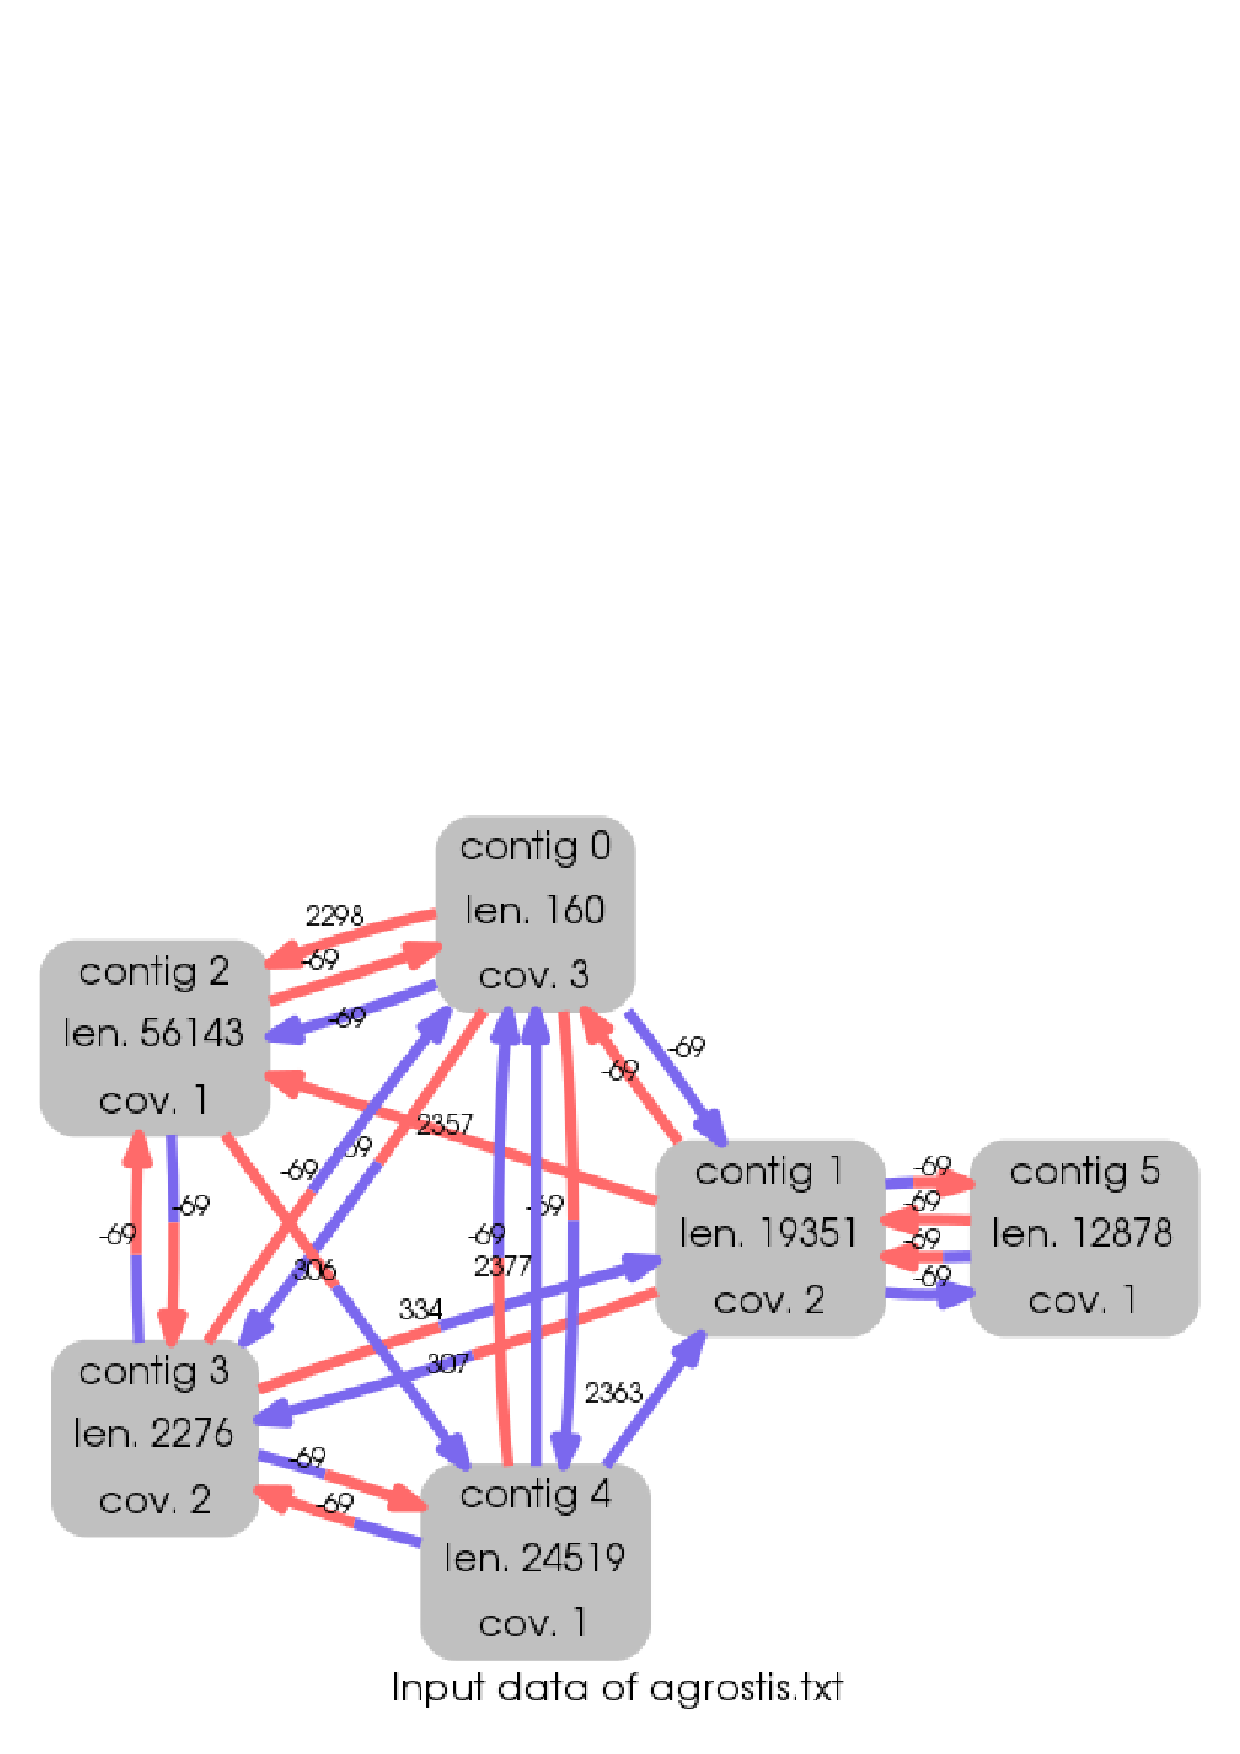
\includegraphics[scale=0.4]{agrostis_INPT}
\caption{Input data of \textit{Agrostis stolonifera} viewed in form of a graph}
{\footnotesize The image was generated with the \textit{graph\_generator.py} script. The color on the links indicate if the links points to the contigs in forward (blue) or reverse (red) orientation.}

\end{figure}

\subsubsection{Other genomes}

%-------------------------------------------------------------------------------
% BODEH!
%-------------------------------------------------------------------------------
\newpage
\subsection{Genscale scaffolding strategy}
\subsection{Benchmarking}
\subsubsection{Published scaffolders chosen for benchmarking}
\subsubsection{Benchmarking strategy}
Chosen scaffolding tools to benchmark against
Benchmarking workflow
Comparisons
QUAST
Comparison function
Visualization
MUMMER
Visualization tool
%-------------------------------------------------------------------------------
% BODEH!
%-------------------------------------------------------------------------------
\section{Results}
\subsection{Data sets compared}
\subsubsection{QUAST and comparison function}
\subsubsection{Visualization}
%-------------------------------------------------------------------------------
% BODEH!
%-------------------------------------------------------------------------------
\section{Conclusion}
\clearpage

%-------------------------------------------------------------------------------
%BIBLIOGRAPHY
%-------------------------------------------------------------------------------

\bibliography{scaffoldingbiblio, scaffoldingbiblio_non_articles}
\bibliographystyle{naturemag}
%\printbibliography
\end{document}